
%----------------------------------------------------------------------------------------
%	PACKAGES AND DOCUMENT CONFIGURATIONS
%----------------------------------------------------------------------------------------

\documentclass{article}

\usepackage[version=3]{mhchem} % Package for chemical equation typesetting
\usepackage{siunitx} % Provides the \SI{}{} and \si{} command for typesetting SI units
\usepackage{graphicx} % Required for the inclusion of images
\usepackage{wrapfig}
\usepackage{natbib} % Required to change bibliography style to APA
\usepackage{amsmath} % Required for some math elements 
\usepackage[utf8]{inputenc}
%\usepackage{natbib}
\graphicspath{ {./images/} }
\setlength\parindent{0pt} % Removes all indentation from paragraphs

\renewcommand{\labelenumi}{\alph{enumi}.} % Make numbering in the enumerate environment by letter rather than number (e.g. section 6)

%\usepackage{times} % Uncomment to use the Times New Roman font

%----------------------------------------------------------------------------------------
%	DOCUMENT INFORMATION
%----------------------------------------------------------------------------------------

\title{Arquitectura de Microcontroladores \\ Practica 1B} % Title


\author{Sergio Hernández Reyes} % Author name

\date{\today} % Date for the report

\begin{document}

\maketitle % Insert the title, author and date



%----------------------------------------------------------------------------------------
%	SECTION 1
%----------------------------------------------------------------------------------------
\section{Objectivo}

Conocer el IDE de desarrollo MPLAB así como sus características y su modo de funcionamiento. En esta práctica se creará un código en C con el fin de encender un led o apagarlo por medio de un switch utilizando el PIC16F15313.



%----------------------------------------------------------------------------------------
%	SECTION 2
%----------------------------------------------------------------------------------------
\section{Desarrollo}
Se crea proyecto con compilador XC8, se crea estructura por medio de Mplab Code Configurator.\\
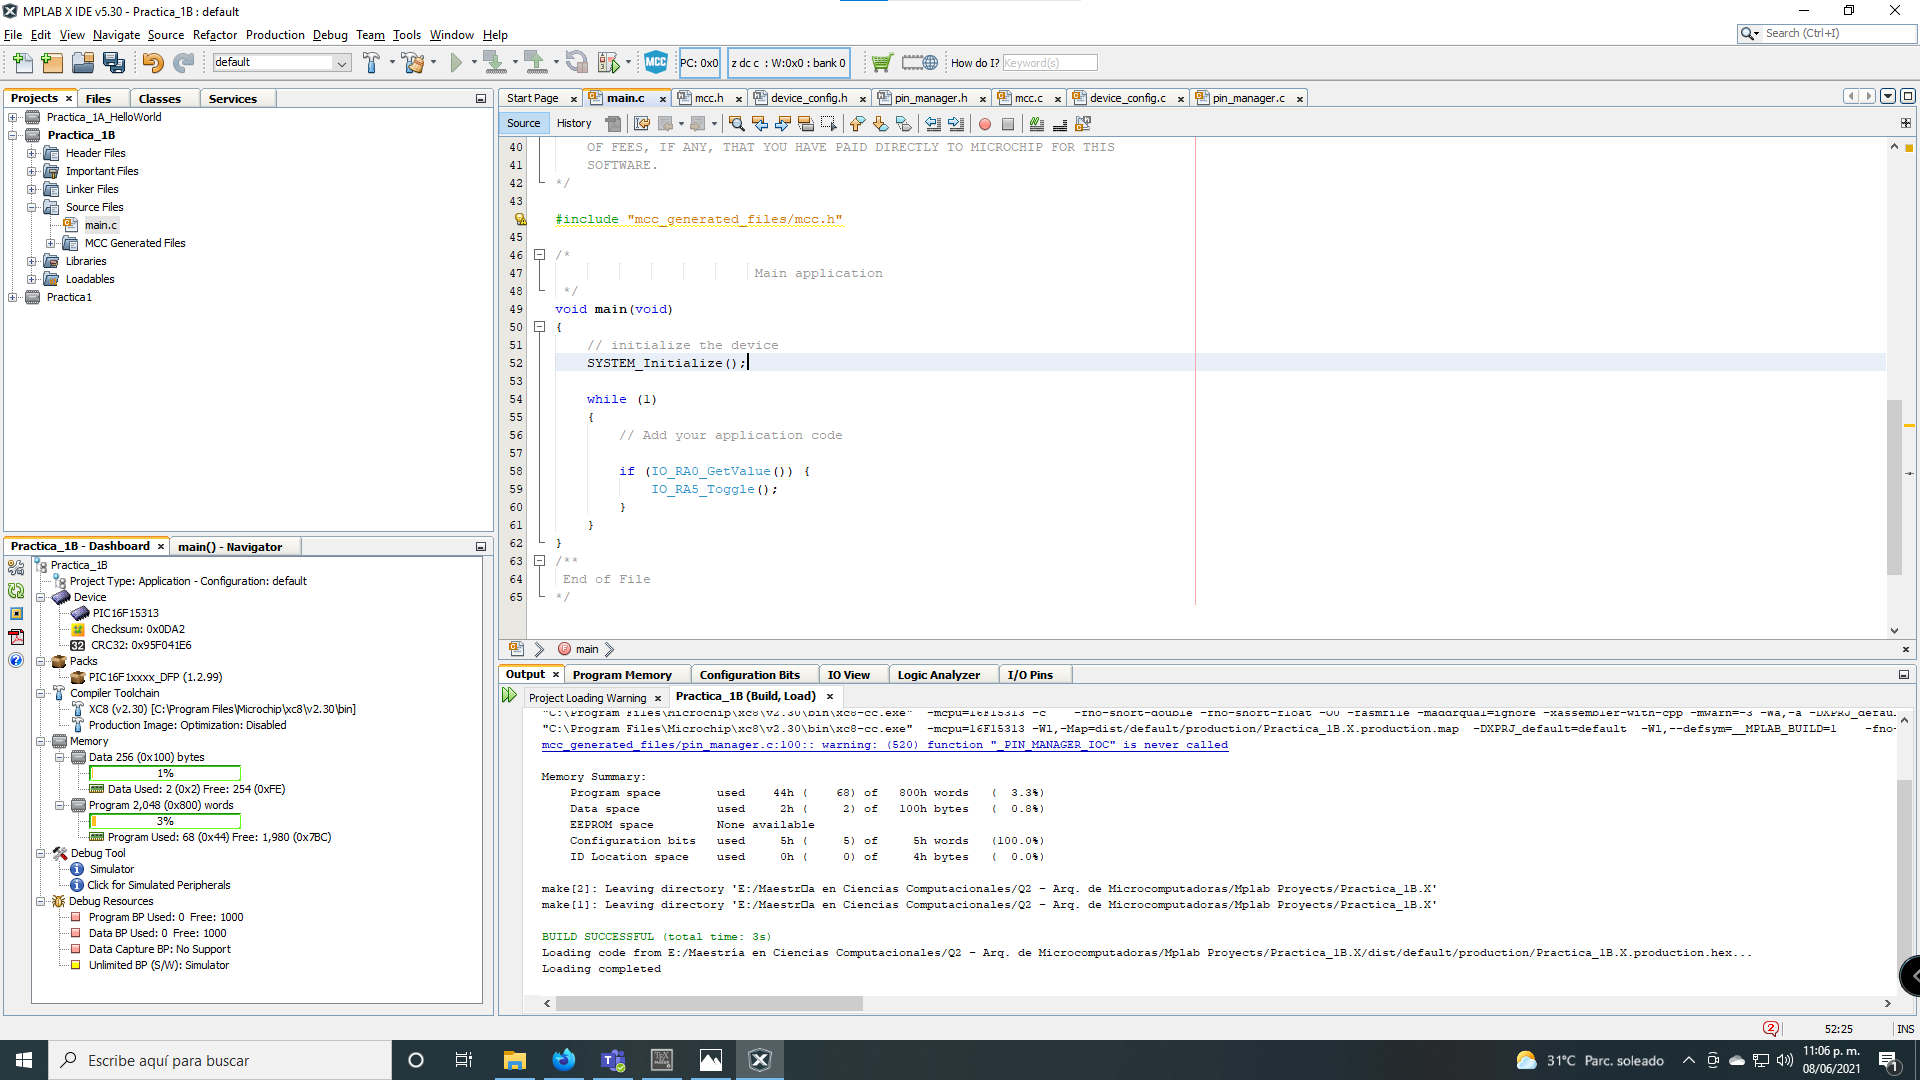
\includegraphics[width=\textwidth]{mplab}\\
\newline
\newline

Se arma circuito para bajar el hexadecimal al microcontrolador por medio del pickit3 y con el uso del MPLAB X Ipe\\
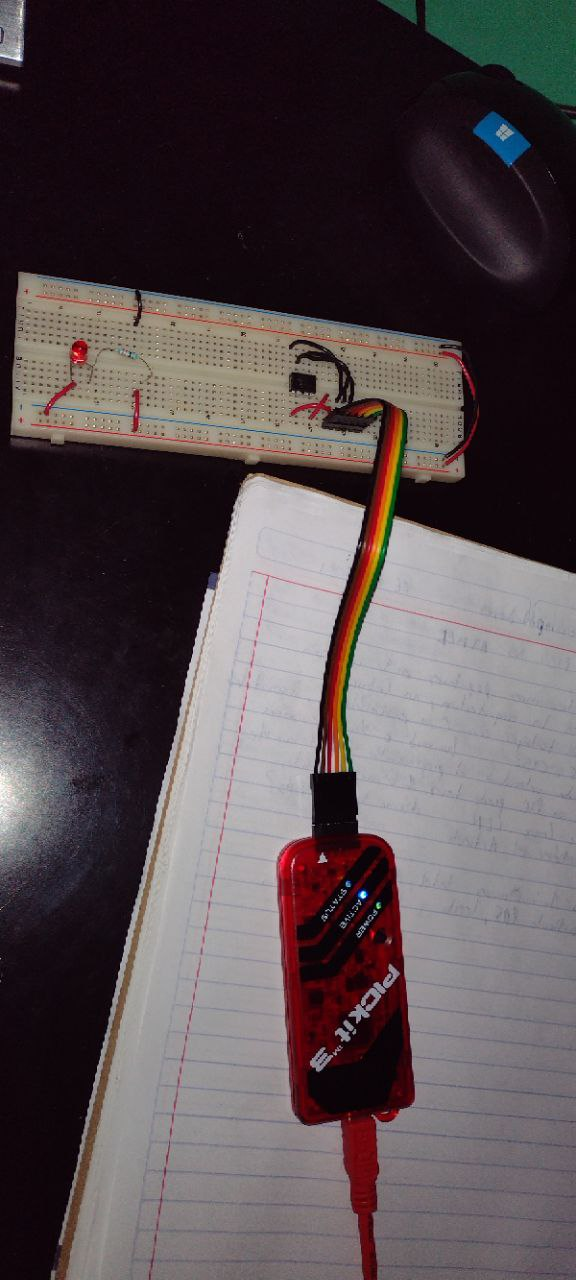
\includegraphics[scale=0.3]{pickit3}\\
\newline
\newline


%----------------------------------------------------------------------------------------
%	SECTION 3
%----------------------------------------------------------------------------------------
\section{Resultados}
Una vez quemado el pic, se procede a armar el circuito que incluye el push boton, el led, y la resistencia correspondiente para poder mostrar el blinking led.\\
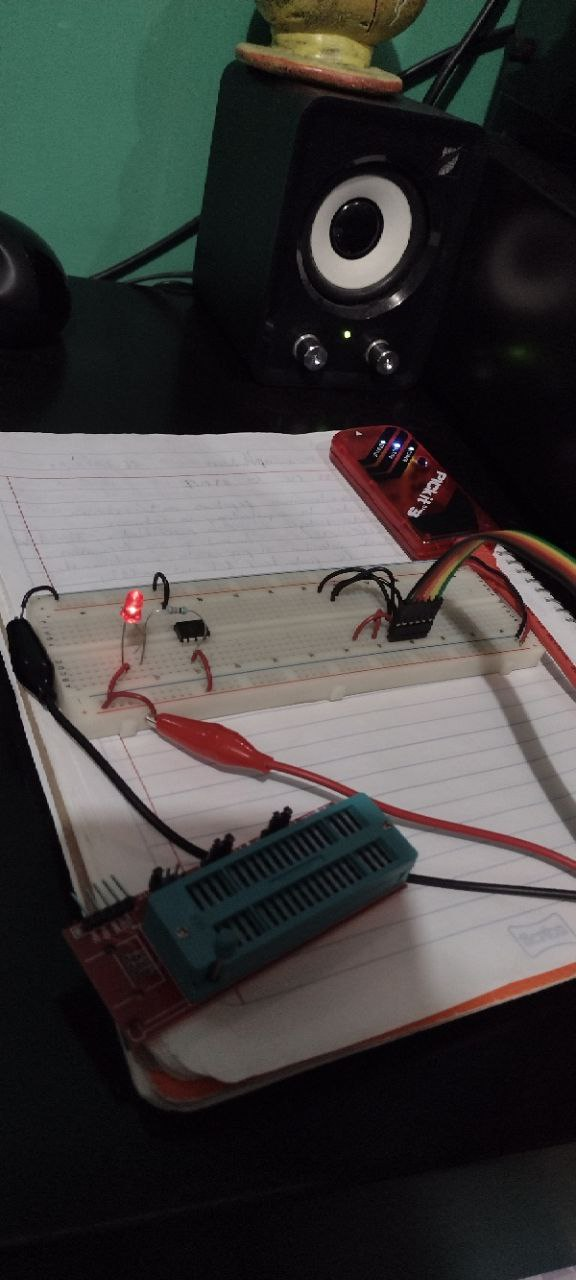
\includegraphics[scale=0.3]{led}\\



%----------------------------------------------------------------------------------------
%	SECTION 4
%----------------------------------------------------------------------------------------
\section{Conclusiones}
Con esta practica pudimos utilizar lo necesario para compilar un código en C y bajarlo a nuestro microcontrolador así como manipular sus entradas y salidas.

%\begin{figure}[h]
%\begin{center}
%\includegraphics[width=0.65\textwidth]{placeholder} % Include the image placeholder.png
%\caption{Figure caption.}
%\end{center}
%\end{figure}
\end{document}